
\documentclass[11pt,dvipdfm]{article}

\usepackage{deauthor}
\usepackage{times}


\usepackage{microtype}
\usepackage{url}
\usepackage{tabularx} %

\usepackage{wrapfig}
\usepackage{array}    %
\usepackage{booktabs}
\usepackage{multicol} %
\usepackage{amsthm} %
\usepackage{appendix}
\usepackage{enumitem}
\usepackage{algorithm2e}
\usepackage{subfigure}
\usepackage{multirow} 
\usepackage{balance}
% \usepackage[normalem]{ulem}
% \let\Bbbk\relax
% \usepackage[dvipdfm]{hyperref}

\usepackage{amsfonts,amssymb}
\usepackage{amsmath,bm}
\usepackage{threeparttable}
\newtheorem{myDef}{Definition}
\usepackage{color}
\usepackage{soul} 
\usepackage{float}
\usepackage{makecell} 
\usepackage{longtable} %
\usepackage{ltablex} %

\usepackage{pifont}
% \usepackage{graphicx}
\usepackage{graphicx}

% \usepackage{fancyhdr}
\usepackage{longtable}
\usepackage{subcaption}

% \theoremstyle{plain}
\newtheorem{examplethm}{Example}[section] 

\newtheorem{theoremthm}{Theorem}[section]
% \newtheorem{example}{Example}[section] 

\definecolor{hiddendraw}{RGB}{205, 44, 36}
\definecolor{hidden-blue}{RGB}{194,232,247}
\definecolor{hidden-orange}{RGB}{243,202,120}
\definecolor{hidden-yellow}{RGB}{242,244,193}
\definecolor{uclablue}{rgb}{0.15, 0.45, 0.68}
% \hypersetup{
%     breaklinks,
%     colorlinks=true,
%     citecolor=uclablue,
%     urlcolor=uclablue,
% }

% \newcommand{\wfj}[1]{\textcolor{blue}{#1}}
% \newcommand{\xzrevision}[1]{\textcolor{blue}{#1}}
\newcommand{\wfj}[1]{{#1}}
\newcommand{\xzrevision}[1]{{#1}}

\title{Evaluating the Factuality of Large Language Models using Large-Scale Knowledge Graphs}


\author{Xiaoze Liu\textsuperscript{$\clubsuit$}, Feijie Wu\textsuperscript{$\clubsuit$}, Tianyang Xu\textsuperscript{$\clubsuit$}, Zhuo Chen\textsuperscript{$\heartsuit$},Yichi Zhang\textsuperscript{$\heartsuit$}, \\ Xiaoqian Wang\textsuperscript{$\clubsuit$}, Jing Gao\textsuperscript{$\clubsuit$}\\
\textsuperscript{$\clubsuit$} Purdue University,
West Lafayette, IN 47907, USA \\
\textsuperscript{$\heartsuit$} Zhejiang University, Hangzhou, China\\
\texttt{\{xiaoze, wu1977, xu1868, joywang, jinggao\}@purdue.edu} \\
\texttt{\{zhuo.chen, zhangyichi2022\}@zju.edu.cn}
}



\newcommand*{\GraphEval}[0]{\textsf{GraphEval}}
\newcommand*{\Truthful}[0]{\textit{Truthful}}
\newcommand*{\Informative}[0]{\textit{Informative}}
\newcommand*{\Correct}[0]{\textit{Correct}}
\newcommand{\removevspace}[1]{}

% \theoremstyle{definition}
% \renewcommand{\paragraph}[1]{\vspace{-1mm}
%     \noindent\textbf{#1.}}

\renewcommand\theadfont{\bfseries} %

\newcommand{\nonsense}[0]{} %


\newcommand{\rmnum}[1]{\romannumeral #1}
\newcommand{\Rmnum}[1]{\expandafter\@slowromancap\romannumeral #1@}

\newcommand{\fix}{\marginpar{FIX}}
\newcommand{\new}{\marginpar{NEW}}



\newcommand{\cz}[1]{{#1}}
\newcommand{\todo}[1]{{ #1}}
\newcommand{\feijie}[1]{#1}

\begin{document}


\maketitle

\begin{abstract}
The advent of Large Language Models (LLMs) has significantly transformed the AI landscape, enhancing machine learning and AI capabilities. Factuality issue is a critical concern for LLMs, as they may generate factually incorrect responses.
In this paper, we propose \GraphEval{} to evaluate an LLM's performance using a substantially large test dataset. Specifically, the test dataset is retrieved from a large knowledge graph with more than 10 million facts without expensive human efforts. Unlike conventional methods that evaluate LLMs based on generated responses, \GraphEval{} streamlines the evaluation process by creating a judge model to estimate the correctness of the answers given by the LLM. Our experiments demonstrate that the judge model's factuality assessment aligns closely with the correctness of the LLM's generated outputs, while also substantially reducing evaluation costs.  Besides, our findings offer valuable insights into LLM performance across different metrics and highlight the potential for future improvements in ensuring the factual integrity of LLM outputs. The code is publicly available at \url{https://github.com/xz-liu/GraphEval}.



\end{abstract}


\section{Introduction}

The rapid progress of Large Language Models (LLMs) has markedly boosted artificial intelligence and machine learning due to their strong contextual text generation capabilities.
\feijie{Despite these groundbreaking advancements, recent works~\cite{EvaluationSurvey, wang2023evaluating} have highlighted the significance of LLMs evaluation.}
\cz{LLMs are prone to producing seemingly authentic yet factually inaccurate responses, a phenomenon known as hallucination~\cite{wang2023survey}. Such errors may stem from outdated or incorrect data during training or the model's learned associations, impacting its reliability.}
\feijie{The evaluation, therefore, helps identify instances of hallucination and understand the LLM's ability to generate coherent and contextually relevant text, i.e., factuality of LLM outputs.}




Recent efforts have been put into the factuality evaluation of LLM. For example, \cite{chen2023felm} introduce FELM, a benchmark comprising diverse factual samples across various domains. Moreover, \cite{tian2023finetuning} and \cite{feng-etal-2023-factkb} utilize external tools (e.g., search engines and a well-trained factual LLM) to estimate the factuality of the generated texts. Representing structured knowledge related to real-world objects, Knowledge Graphs (KGs) \cite{auer2007dbpedia, bollacker2008freebase, suchanek2007yago, carlson2010toward} have gained prominence for LLM factuality assessments. They primarily originate from Wikipedia, encapsulate factual information for AI tasks, and form the knowledge base with datasets like Natural Questions \cite{NaturalQuestions}. 


\pagebreak
Several studies \cite{sun2023head,liang2023holistic} have focused on creating benchmarks from knowledge sources by posing factual questions derived from triples in \cz{KGs}. %
These methods, as depicted in the left part of Figure \ref{fig:intro_demo}, either (i) sample subgraphs from large KGs or (ii) extract a subset of knowledge from text documents to construct multiple-choice or text question-answer pairs. Those question pairs are then posed to LLMs to assess their factuality.
However, the above-mentioned methods or evaluation strategies face challenges in comprehensively evaluating the factuality of LLMs. 
{\it Firstly}, \cz{the scope of evaluation data is often limited or incomplete, focusing predominantly on specific domains.}
\cz{This limitation restricts the evaluation's breadth and undermines its applicability across various contexts, failing to cover the wide range of topics LLMs are expected to handle.}
The specialized nature of these datasets means that the evaluation may not accurately reflect the model's performance in generating factual content across a broader spectrum of subjects. {\it Secondly}, the process of factuality evaluation itself is inherently time-consuming and costly. It necessitates that an LLM generate full texts, which must then be meticulously assessed for accuracy and reliability. 
\cz{This comprehensive generation and detailed review demand significant computational resources and extensive human effort~\cite{wang2023evaluating} for validation.}
As a result, the process becomes less feasible for regular or large-scale applications, limiting the frequency and scope of 
\cz{practical evaluations}.
{\it Lastly}, due to the limited size of the evaluation data, there may be biases in the benchmarks~\cite{gallegos2023bias}, or risks of test data leakage \cite{zhou2023dont}, which might compromise the validity of the evaluations.
Together, these challenges underscore the need for more scalable, efficient, and domain-agnostic approaches to evaluating the factuality of LLM-generated texts.




To this end, we propose \GraphEval{}, which consists of two novel features in terms of the design, as presented on the right side of Figure \ref{fig:intro_demo}. First, we utilize \cz{KGs} that encapsulate factual information sourced from verifiable content like Wikipedia. With the KG, millions of prompts can be automatically generated, leading to a significant saving of human efforts in labeling the ground truth. From the data perspective, the KG gives a more diversified and comprehensive evaluation of the LLMs' factuality. Second, the proposed method efficiently reduces the computation costs and speeds up the evaluation process. Specifically, we incorporate a highly reliable and lightweight judge model to decide whether an LLM can generate an accurate response to a designated question. 
Instead of generating the full text, the judge model returns three options (i.e., True, False, and I don't know) to simulate LLMs' responses to a given prompt. To ensure the reliability of the simulated results, the judge model is trained based on a few question-answer pairs, where the questions are sampled from KGs and the answers are generated by the target LLM. As a result, the judge model can serve as a replacement for the factuality evaluation of the facts extracted from large-scale KGs.   In summary, our contributions are as follows:



  

\begin{figure}[t]
    \centering 
    \includegraphics[width=.97\textwidth] {submissions/Jing2024/figures/intro_example.pdf} 
    \vspace{-2mm} 
    \caption{\feijie{Existing works compared to the proposed \GraphEval{} on factuality evaluation.}} 
    \vspace{-4mm}
    \label{fig:intro_demo}
\end{figure}  

\begin{itemize}[topsep=0pt,itemsep=0pt,parsep=0pt,partopsep=0pt,leftmargin=*]
    \item We propose \GraphEval{}, a large-scale evaluation framework that assesses the factuality of LLMs using KGs. \GraphEval{} evaluates the factuality of LLMs using the entire KGs, providing a more diversified and comprehensive evaluation of the LLMs' factuality.
    \item We introduce a judge model to assist with the evaluation process, which reduces the computational cost and enhances the efficiency of the evaluation. We also give a theoretical analysis of the judge model to demonstrate its validity.
    \item We conduct extensive experiments on a large-scale KG, i.e., DBpedia, to demonstrate the effectiveness and efficiency of \GraphEval{} in evaluating the factuality of LLMs.
    \item We provide an in-depth analysis of the LLM's performance on the KGs, including the LLM's performance with respect to relation types, head entity types, tail entity types, and the relation of LLM performance to degree and pageviews. 
\end{itemize}
     

\vspace{-2mm}
\section{Related Work}
\vspace{-2mm}
\paragraph{\cz{Factuality Issue of LLMs}}
Factuality issue~\cite{wang2023survey, zhang2023siren}, is the issue that LLMs may produce content inconsistent with established facts. As outlined in~\cite{wang2023survey}, this issue may be due to: \cz{\textbf{\textit{(\rmnum{1})}}} LLMs lacking expertise in specific domains~\cite{ScienceQA,bolton2024biomedlm}; \cz{\textbf{\textit{(\rmnum{2})}}} LLMs' unawareness of recent developments or changes~\cite{TempQuestions,yao2023editing}; \cz{\textbf{\textit{(\rmnum{3})}}} LLMs not retaining~\cite{wang2023evaluating,TQ,NaturalQuestions} or forgetting~\cite{goodfellow2015empirical,kotha2023understanding,wang2022preserving, chen2020recall, zhai2023investigating} knowledge from its training corpus; and \cz{\textbf{\textit{(\rmnum{4})}}} LLMs failing to reason with the knowledge they possess~\cite{liu2023we, berglund2023reversal,tan2023chatgpt}. The factuality issue has been addressed by various works, by incorporating Retrieval Augmented Generation (RAG)~\cite{lewis2020retrieval, wang2024blendfilter}, fine-tuning~\cite{tian2023finetuning}, and knowledge-enhanced models~\cite{feng-etal-2023-factkb,diao2023mixtureofdomainadapters}. 
To summarize, these approaches integrate other knowledge sources into the LLMs' training process or use them to augment the models' knowledge base, thus alleviating the factuality issue. Our work differ from them in that we evaluate the factuality of LLMs, rather than providing factuality enhancement methods.


\paragraph{\cz{Factuality Evaluation of LLMs}}
The expanding use of LLMs across various domains necessitates the assurance of their output's accuracy and reliability. 
A range of benchmarks and evaluation methodologies for assessing large language models (LLMs) are proposed.
These works primarily focus on evaluating the factuality, truthfulness, reasoning capabilities, and adaptability to new information of LLMs. MMLU~\cite{MMLU} and TruthfulQA \cite{TruthfulQA} aim to measure the factuality and truthfulness of LLMs across diverse tasks, while C-Eval \cite{C-Eval} focuses on the Chinese context, assessing models' knowledge of Chinese culture and laws.
%  BigBench  \cite{BigBench} challenges LLMs with tasks beyond current capabilities, and HaluEval \cite{HaluEval}, SelfAware \cite{yin-etal-2023-large}.
% , and the Pinocchio \cite{Pinocchio} benchmark explore models' propensity for generating hallucinations, their self-awareness, and their reasoning skills, respectively. REALTIMEQA  \cite{kasai2022realtimeqa} and FreshQA  \cite{vu2023freshllms} introduce dynamic benchmarks that test LLMs on current events and up-to-date knowledge.
 There are also works \cite{sun2023head, liang2023holistic} that propose factuality evaluation using subsets of KGs. %
However, selecting subsets of KGs to test LLMs can introduce selection bias. For example, random sampling can focus more on a few popular domains or subjects more densely connected with others, thus not showing LLMs' factuality on diversified topics.
Our work addresses this limitation by %
proposing a resource-efficient method to evaluate the factuality of LLMs which allows evaluations on whole KGs instead of subsets, thus providing a more diversified and comprehensive evaluation of the LLMs' factuality, enabling an extensive assessment of LLM's factuality and reasoning abilities in a way that existing individual benchmarks do not as they only focus on specific aspects. 


\paragraph{\cz{Using KGs in LLMs}}
\cz{KGs} are structured representations of factual knowledge, typically in the form of (head, relation, tail) triples.  There are lots of efforts in constructing \cite{auer2007dbpedia}, and reasoning~\cite{bordes2013translating} on KGs. This has made KGs an indispensable resource of factual knowledge for AI tasks. 
Currently, the most common way of integrating KGs with LLMs is using KGs as an external knowledge source to enhance LLM performance by pre-training, fine-tuning, or in-context learning~\cite{yasunaga2022deep,jiang-etal-2023-reasoninglm, zhang2024knowledge,kim2023kggpt,luo2023reasoning}. Our work is different from these works in that we use KGs to evaluate the factuality of LLMs, rather than enhancing the LLMs with KGs. 




%!TEX root=../2022_IEEE_DEB_Vizier.tex

% %%%%%%%%%%%%%%%%%%%%%%%%%%%%%%%%%%%%%%%%
% \begin{figure}[t]
%   \centering
%   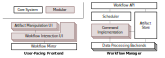
\includegraphics[width=0.7\textwidth]{graphics/systemarch}\\[-5mm]
%   \caption{Vizier's architecture, comprised of a user-facing frontend component and a backend component.}\label{fig:vizier-architecture}
% \end{figure}
% %%%%%%%%%%%%%%%%%%%%%%%%%%%%%%%%%%%%%%%%

%%%%%%%%%%%%%%%%%%%%%%%%%%%%%%%%%%%%%%%%%%%%%%%%%%%%%%%%%%%%%%%%%%%%%%%%%%%%%%%%
\pagebreak[4]
\subsection{Solution Overview}
\label{sec:solution-overview}

%%%%%%%%%%%%%%%%%%%%%%%%%%%%%%%%%%%%%%%%
\begin{wrapfigure}[12]{r}[0pt]{12cm}
  \centering
  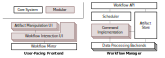
\includegraphics[width=0.7\textwidth]{graphics/systemarch}\\[-5mm]
  \caption{Vizier's architecture, comprised of a user-facing frontend component and a backend component.}\label{fig:vizier-architecture}
\end{wrapfigure}
%%%%%%%%%%%%%%%%%%%%%%%%%%%%%%%%%%%%%%%%
An overview of Vizier's architecture is shown in \Cref{fig:vizier-architecture}.
Addressing requirement \textbf{W1}, the central abstraction in Vizier is a workflow: a linear sequence of steps. % taken by the user in pursuit of a specific objective.
Unlike classical workflow systems, Vizier does not require users to explicitly declare information flow between steps.
Rather Vizier borrows the model employed in popular computational notebooks like Jupyter, where inter-cell communication occurs through a global state (artifacts) passed sequentially through steps.
Following notebook conventions, we refer to these steps as \emph{cells}, and the global state as a \emph{scope}, a map from artifact name to the version of the artifact valid at this point in the workflow. Vizier stores artifacts in common formats through a versioned \textbf{Artifact Store} (\Cref{sec:data-artifacts}), addressing requirement \textbf{A2}.
In \Cref{sec:vizier-workflows}, we formalize Vizier's workflow model, and show how we satisfy requirement \textbf{W3} by instrumenting how each cell interacts with the scope, allowing us to determine what artifact versions are valid.

Vizier's workflow semantics, paired with the versioned artifact store and workflow versioning (\Cref{sec:vizier-history}) addresses requirement \textbf{W2}. % as notebooks have a natural concept of logical order (the order of cells in the notebook) that can be adjusted over time.
% Adding workflow versioning  is sufficient to fully address the requirement.
In contrast, classical notebooks like Jupyter or Zeppelin rely on the global state of an interpreter for inter-cell communication.
Reverting this state to an earlier revision is challenging~\cite{zelnicki:2017:nodebook}, limiting their ability to satisfy requirement \textbf{W3}.
Vizier instead relies on its versioning system, allowing its \textbf{Scheduler} to automatically detect and re-evaluate stale cells (\Cref{sec:vizier-scheduler}).
To address requirement \textbf{A3}, we designed a light-weight uncertain data model that is implemented in Vizier in the form of \textit{caveats}, annotations on data that indicate uncertain values and rows  (\Cref{sec:data-docum-error}).

Addressing requirement \textbf{A1} requires modularity in both Vizier's front- and back-end components.
First, the user's interactions with a workflow and artifacts, whether through a scripting language, graphical interaction, or any other modality, need to be captured for replay (simultaneously addressing requirement \textbf{A4}). In Vizier this is achieved by requiring that every update to an artifact made through a particular modality has to be reflected as an operation in the workflow, i.e., a data update is translated into a workflow update.
Vizier manages a collection of \textbf{Command Implementations} that implement the logic behind these artifact transformations (\Cref{sec:multimodality}).
To streamline the implementation of commands, Vizier's data formats and transformations are built over standard \textbf{Data Processing Backends} like Apache Spark.
% For example, Vizier supports fine-grained provenance over datasets by encoding them as Spark data frames.

The frontend is implemented over a \textbf{Workflow Mirror} that uses websockets to reflect a live view of the workflow the user is editing.
Vizier automatically derives a default \textbf{Artifact Manipulation User Interface} for its notebook interface from each command's parameter schemas. This interface suffices for many templated commands, but the frontend can be further extended to provide a more customized experience, for example for Spreadsheet-style direct manipulation of data (\Cref{sec:spreadsheets}).
As illustrated in \Cref{fig:screenshot}, the frontend displays three \textbf{Workflow Interaction User Interfaces} by default: (i) A direct display of the workflow as a notebook, (ii) a table of contents summary of the notebook, including highlighting from documentation, and (iii) a list of artifacts derived by the notebook.
Several of these components, including the notebook and the artifact list provide access to direct manipulation interfaces.
Additional views currently implemented in Vizier include: (iv) A caveat view (\Cref{sec:data-docum-error}) that shows and tracks potential errors in the workflow and data, (v) a history view that shows the evolution of the workflow over time, and (vi) a data provenance subway diagram view.

%%%%%%%%%%%%%%%%%%%%%%%%%%%%%%%%%%%%%%%%%%%%%%%%%%%%%%%%%%%%%%%%%%%%%%%%%%%%%%%%
\begin{figure}
  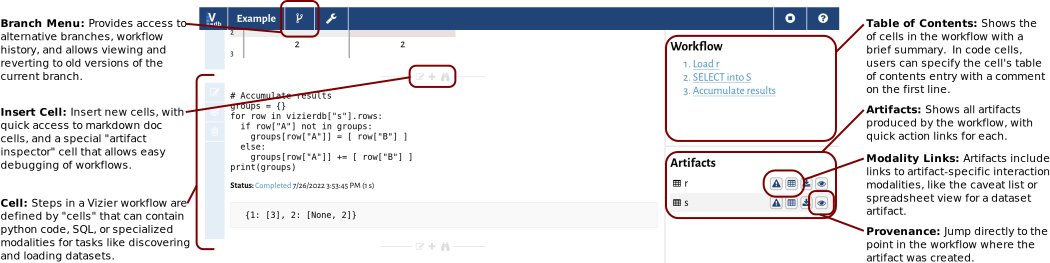
\includegraphics[width=\textwidth]{graphics/screenshot.pdf} 
  \caption{The Vizier User Interface}
  \label{fig:screenshot}
\end{figure}
%%%%%%%%%%%%%%%%%%%%%%%%%%%%%%%%%%%%%%%%%%%%%%%%%%%%%%%%%%%%%%%%%%%%%%%%%%%%%%%%

%%% Local Variables:
%%% mode: latex
%%% TeX-master: "../2022_IEEE_DEB_Vizier"
%%% End:


\section{Method}

% \vspace{-3mm}
\GraphEval{} is designed to measure the factuality of a language model in relation to a \cz{KG}. As presented in Figure \ref{fig:framework}, the proposed work is divided into three steps: 
\begin{itemize}[topsep=0pt,itemsep=0pt,parsep=0pt,partopsep=0pt,leftmargin=*]
    \item \textbf{Step 1: Question and label collection from KGs and LLMs. } \quad  The model samples triples from KGs and converts each triple into a declarative statement with GPT-4-crafted templates. To prepare versatile statements, we employ \textit{negative sampling}, where incorrect statements are intentionally generated. Afterward, those statements are posed to collect the labels answered by an LLM (i.e., Yes, No, and I don't know (IDK)).
    \item \textbf{Step 2: Judge model training.} \quad With the triples collected in the first step, we train a judge model to avoid long-generated texts and conserve computational resources. In detail, inspired by~\cite{azaria-mitchell-2023-internal}, we train a classifier with LLMs' hidden states to make a selection within the above three options. We also apply p-tuning \cite{liu2021p} to minimize the prompt/instruction size.
    \item \textbf{Step 3: Evaluation on whole KGs.} \quad Similar to the first step, we retrieve all true/false statements from KGs. Subsequently, these statements are fed into the trained judge model to estimate the factuality of LLM. This process enables a thorough and multifaceted analysis of the LLM's performance in terms of factuality, drawing from a wide range of perspectives to provide a more comprehensive and diversified evaluation.
\end{itemize}
In the following sections, we will discuss the details of each step. 

\subsection{Question and Label Collection}
\label{sec:question_generation}

\paragraph{Question Generation}
In order to evaluate the language model's ability to identify false statements, we directly construct a declarative sentence for each triple. This addresses the ineffectiveness of multiple-choice questions in our task. %
Firstly, multiple-choice prompts may cause misalignment with parametric knowledge in LLMs. Since LLMs mainly learn parametric knowledge through text data, in which knowledge facts are mostly represented as declarative sentences~\cite{weller2023according}, employing multiple-choice questions may hinder the evaluation of factuality. Secondly, multiple-choice questions have more complex labels (i.e. A, B, C, D) than declarative sentences (i.e. True, False, IDK), which can complicate the tasks for the judge model, influencing the overall effectiveness. We use an example to illustrate this.

\begin{examplethm}
    For the triple \texttt{(Barack Obama, birthPlace, Hawaii)}, a multi-choice question can be generated as \texttt{Where was Barack Obama born?} with choices \texttt{A. Hawaii B. Chicago C. New York D. Los Angeles}. Here, for the same triple, we can also generate another multi-choice question as \texttt{Where was Barack Obama born?} with choices \texttt{A. China, B. Hawaii, C. Japan, D. Russia}. The two questions represent the same triple, but the choices are different. %
    As mentioned in the last paragraph, this can introduce complexity and potential misalignment with an LLM’s training and result in inconsistent responses. %
    
\end{examplethm}

To address the ineffectiveness of multiple-choice questions, we propose to directly ask the LLMs whether a statement is true or not.
For instance, considering the triple \texttt{(Barack Obama, birthPlace, Hawaii)}, we can formulate a fact \texttt{Obama was born in Hawaii} by integrating the entities \texttt{Barack Obama} and \texttt{Hawaii} into the template \texttt{ \{head\} was born in \{tail\}}. %
Each template corresponds to the relation of a triple, and they are crafted to be clear and straightforward statements. GPT-4 is employed to generate these templates for all relations in the \cz{KG}. 
 These generated templates are then manually reviewed and refined to ensure their compatibility with the \cz{KG}. Then, we can ask a question to the LLMs, such as \texttt{Is the statement "Barack Obama was born in Hawaii" true or false?}.
    Here, the templates are corresponding to the relations of the triples. This is because the number of relations in the \cz{KG} is limited, while the number of triples is large. Therefore, we can use the relations to categorize the triples, and then use the templates to generate questions for each category. This can significantly reduce human labor, i.e., monitoring less than 1000 templates compared with monitoring more than 10 million triples.
See the Appendix~\ref{app:detailed_settings} for the detailed settings of the relation templates.

\paragraph{Negative sampling}
Although the declarative sentences simplify the training of the judge model, they alone are insufficient to evaluate the language model's factual accuracy. LLMs can simply answer true for every question, and still get a high accuracy. %
To address this, we introduce negative sampling, a technique commonly used in \cz{KG} completion tasks, to generate false statements. Specifically, we randomly replace one entity or relation in the original triple with another entity or relation sampled from the \cz{KG}. For example, given the triple \texttt{(Barack Obama, birthPlace, Hawaii)}, we can replace the tail entity \texttt{Hawaii} with another entity \texttt{Chicago} to form the false statement \texttt{Barack Obama was born in Chicago}. These false statements are then presented to the LLMs to evaluate their ability to identify falsehoods.

\vspace{-2mm}
\subsection{Judge Model}\label{method:judge}

% \vspace{-2mm}
% \wfj{\paragraph{Motivations} }

\vspace{-2mm}
Normally, to evaluate the factual accuracy of a language model, we would generate questions from a \cz{KG} and then pose these questions to the language model. However, given the expansive nature of \cz{KG}s, it's impractical to label every generated question by the LLM. 
A more efficient approach is to use the last token logits of the LLMs as their answers. However, %
recent research has highlighted discrepancies between these logits and the model's actual text outputs~\cite{wang2024myanswer}. 
Therefore, we introduce a novel judge model to assist with this task. The judge model, initially trained on a subset of labeled questions, is then employed to label the remaining questions. Uniquely, inspired by ~\cite{azaria-mitchell-2023-internal}, the judge model utilizes the LLM's hidden state as input, as a replacement of the LLM's last layer with compressed output tokens. Specifically, three output classes are used: \textit{True}, \textit{False}, and \textit{I don't know}. The judge model is a two-layer feed-forward neural network, with a layer normalization and a ReLU activation function. 
This approach diverges from standard practices where LLMs generate answers, as here we only forward the transformer once. Consequently, this operation is significantly less resource-intensive than full answer generation, allowing the judge model to efficiently process a large number of questions with limited labeled data.
% \vspace{-2mm}
\wfj{With this model, we can glance at the correctness of an LLM, i.e., how likely the model can answer a question relevantly and correctly. We evaluate the performance of the judge model using two metrics: (i) \textit{Truthfulness}, i.e., the likelihood that the judge model prediction matches the LLM correctness under a given question; and (ii) \textit{Informativeness}, i.e., the likelihood that the judge model does not give a prediction of `I don't know.' 
% Clarifying question on Page 5: Why were "truthfulness," "informativeness," and "correctness" prioritized over other possible metrics like "relevance"? OR “correctness” is like “relevance”?
Since the evaluation is based on a general KG that spans multiple domains, other metrics such as ``Relevance'' would typically require a more specific contextual framework. Nonetheless, future research could explore the use of more context-specific metrics tailored to the LLM's domain of application.
}

\vspace{-2mm}
\paragraph{Efficiency}
To further enhance the judge model's efficiency, we include 2 extra components. First, we found that the instruction prefix of the LLMs is too large for the judge model to process efficiently. We thus fine-tune a {\it prompt encoder}~\cite{liu-etal-2022-p} to reduce the large input of the prompt prefix, which would be the same for all questions. 
Second, we found that our judge model, with the training process on the labeled dataset, is robust to the LLM's hidden states. %
In experiments, we observed that our judge model can seamlessly utilize hidden states from distinct LLMs without significant differences in performance. For instance, within the LLaMA 2 model family, which contains 3 models with different parameters: 7B, 13B, and 70B, we found that the judge model's performance is consistent regardless of whether the hidden states are from 7B, 13B, or 70B. %
Therefore, we can use the model with the least parameters, as a {\it substitute model} when computing the hidden states. This gives us a huge reduction in computational cost.






\paragraph{Analysis of Judge model}
In this part, we assume there are two datasets; one is for training the judge model, and the other is for evaluation, denoted by $\mathcal{D}_S$ and $\mathcal{D}_T$, respectively. As the proposed judge model leads to a triple classification task, we assume a hypothesis portfolio $h = \{h_t, h_f, h_{idk}\}$, where these three hypotheses separately predict if a sample can be correctly answered by the LLM, i.e., True, False, and IDK. In other words, the hypothesis $\hat{h} \in h$ maps an input $\mathbf{x}$ to $\{0, 1\}$, where $1$ means the input satisfies the hypothesis conditions. For a given input $\mathbf{x}$, the equality 
$h(\mathbf{x}) = h_t(\mathbf{x}) + h_f(\mathbf{x}) + h_{idk}(\mathbf{x}) = 1$
always holds because the judge model provides an only output. Define the convex loss function for a hypothesis $\hat{h} \in h$ to be $$L_{\mathcal{D}}(\hat{h}) = \sum_{(\mathbf{x}, y) \in \mathcal{D}} |\hat{h}(\mathbf{x}) - \boldsymbol{1}_{\hat{h}}(y)|,$$ where $\boldsymbol{1}_{\hat{h}}(y)$ indicates if the data indeed satisfies the hypothesis. Since a wrong prediction for data $(\mathbf{x}, y)$ results in $\sum_{\hat{h} \in h} |\hat{h}(\mathbf{x}) - \boldsymbol{1}_{\hat{h}}(y)| = 2$, we define the misclassification rate as 
$$L_{\mathcal{D}} \left(h\right) = \frac{1}{2} \left(L_{\mathcal{D}} \left(h_t\right) + L_{\mathcal{D}} \left(h_f\right) + L_{\mathcal{D}} \left(h_{idk}\right)\right) $$ 

Below is a theoretical analysis to understand the bound of the misclassification rate, which is driven by Theorem 2 of \cite{ben2010theory}.

\begin{theoremthm}
Let $\mathcal{H} = \{\mathcal{H}_t, \mathcal{H}_f, \mathcal{H}_{idk}\}$ be a set of hypothesis spaces of VC dimension $d$. If $\mathcal{U}_S, \mathcal{U}_T$ are the samples of size $m$ each, drawn from $\mathcal{D}_S$ and $\mathcal{D}_T$, respectively, then for any $\delta \in (0, 1)$, with probability at least $1-\delta$, for every $h \in \mathcal{H}$, we have
\begin{equation}
    L_{\mathcal{D}_T} \left(h\right) \leq L_{\mathcal{D}_S} \left(h\right) + \frac{3}{4} d_{\mathcal{H} \Delta\mathcal{H}} \left(\mathcal{U}_S, \mathcal{U}_T\right) + 6 \sqrt{\frac{2d \log \left(2m\right) + \log\left(2/\delta\right)}{m}} + \frac{1}{2} \lambda
\end{equation}
where $\lambda = \inf_{h \in \mathcal{H}} \left(L_{\mathcal{D}_S}\left(h\right) + L_{\mathcal{D}_T}\left(h\right)\right)$ is the optimal combined error, $d_{\mathcal{H} \Delta\mathcal{H}}$ measures the distribution discrepancy between two distributions. 
\end{theoremthm}
\feijie{The above theorem provides insights for the generalization bound of the judge model. The bound is associated with the discrepancy between training data $\mathcal{D}_S$ and evaluation data $\mathcal{D}_T$, and the discrepancy can be measured by drawing samples from both training and evaluation datasets for an equivalent size. Moreover, the bound is affected by the optimal hypothesis over all the data, i.e., $\mathcal{D}_S \cup \mathcal{D}_T$, where a lower error leads to improved performance of the judge model.}



\subsection{Evaluation}


For evaluating the LLM's performance, we consider \textit{Correctness}, which is defined as the proportion of questions for which the LLM's response matches the true label (or false label if the question is generated from a negative triple). This captures the accuracy of the LLM in identifying correct information and distinguishing it from fabricated (negative) triples.
We also adopt the metrics of \textit{Truthfulness} and \textit{Informativeness}, as defined in \cite{TruthfulQA}. \textit{Truthfulness} refers to the likelihood of the language model (LLM) providing an honest response. A response is considered \Truthful{} if the LLM either provides the correct answer or opts for `I don't know'. This criterion assesses the model's ability to be honest about what it knows and to admit uncertainty rather than making false statements. \textit{Informativeness} is the probability of the LLM offering any substantive information, irrespective of its accuracy. An answer is deemed \Informative{} if it is anything other than `I don't know'. This reflects the model's capacity to provide substantial information without resorting to uncertainty or avoidance of an answer. 

When considering multiple negative triples sampled, we combine the results for all negative triples sampled from a triple $\tau$, as well as the results for their original positive triple $\tau$, to calculate the overall performance of the LLM. 
Since correctly detecting a real triple from KG is much simpler than detecting a negative triple, we want to give a max penalty to the LLM's wrong response to the real triple when designing the metric. Therefore, if a real triple is predicted as false, the LLM will score $0$ across all metrics. Then, the negative triple results are averaged to give a fine-grained evaluation of the LLM's performance.
To achieve this, for each performance metric, we define functions $\mathcal{F}$ which evaluates the LLM's response to $\tau$ and $\mathcal{F}'$  to each negative triple $\tau'$ sampled from $\tau$. The overall performance metric for $\tau$ is then calculated as:
\begin{equation}
\text{Metric}(\tau) = \max\left(0, \mathcal{F}(\tau) - \frac{1}{|\mathcal{N}(\tau)|}
\sum_{\tau' \in \mathcal{N}(\tau)} \mathcal{F}'(\tau')\right)
\end{equation}
Here, $\mathcal{N}(\tau)$ represents the set of all negative triples generated from the positive triple $\tau$. $\mathcal{F}$  and $\mathcal{F}'$ are defined as follows: \cz{\textbf{\textit{(\rmnum{1})}}} {\it Correctness.}
    $\mathcal{F}$ is defined such that it is $1$ if the judge model predicts that a real (positive) triple is True, and it is $0$ otherwise; $\mathcal{F}'$ is 0 if the judge model predicts a negative triple as False, and 1 otherwise. 
    \cz{\textbf{\textit{(\rmnum{2})}}} {\it Truthfulness.}
    When measuring \textit{Truthfulness}, $\mathcal{F}$ is set to $1$ if the judge model's prediction for the input $\tau$ is either True or IDK, and it is $0$ otherwise. Similarly, $\mathcal{F}'$ is set to $1$ if the judge model's prediction for the input $\tau'$ is True, and $0$ otherwise; and 
    \cz{\textbf{\textit{(\rmnum{3})}}} {\it Informativeness.}
    For \textit{Informativeness}, $\mathcal{F}$ is defined as $1$ if the judge model's prediction for the input $\tau$ is anything other than "I don't know", and it is $0$ otherwise. $\mathcal{F}'$ is set to $1-\mathcal{F}$ on the informativeness metric.
By applying this equation, we can systematically compute the \textit{Correctness}, \textit{Truthfulness}, and \textit{Informativeness} of an LLM's responses in a consistent and comprehensive manner, offering a detailed insight into its overall performance. 



 














\section{Experiments}

\subsection{Experiment Setup}





\paragraph{Data}
We use DBpedia~\cite{auer2007dbpedia}, a large-scale knowledge graph constructed from Wikipedia. 
We report the statistics of the DBpedia knowledge graph in Table \ref{tab:dbpedia_stat}.  Note that there are ``dummy'' entities in DBpedia that represent a fact that is only true on a specific time period. An example is \url{https://dbpedia.org/page/Kathy\_Greenlee\_\_Tenure\_\_1}. For simplicity, we remove these dummy entities and triples related from the knowledge graph. We refer to the remaining triples as the DBpedia knowledge graph. The DBpedia knowledge graph contains 4,928,232 entities, 633 relations, and 16,915,848 triples. The average node degree of the knowledge graph is 6.80, and the density of the knowledge graph is $7.18\times 10^{-7}$. 

\begin{table}[t]
\centering\small
\begin{tabular}{c|c|c|c|c}
\toprule
\textbf{\#Entities} & \textbf{\#Relations} & \textbf{\#Triples} &  \textbf{Avg. degree} & \textbf{Density} \\ \midrule
4,928,232 & 633 & 16,915,848 & 6.80 & $7.18\times 10^{-7}$ \\ \bottomrule
\end{tabular}
\vspace{-2mm}
\caption{Statistics of the DBpedia knowledge graph.}
\label{tab:dbpedia_stat}
\vspace{-5mm}
\end{table}




 
   

\paragraph{LLMs}
In this paper, we evaluate the Meta LLaMA 2 family~\cite{touvron2023llama}, including LLaMA-2-7B, LLaMA-2-13B, and LLaMA-2-70B, and Google's Gemma~\cite{gemmateam2024gemma} including Gemma-2B and Gemma-7B. 
For each language model, we first randomly sample 2000 triples, and perform a negative sampling to obtain another 2000 negative triples. For each triple, we ask the LLM 3 times the same question, on whether the triple is true, false, or the LLM doesn't know. We use majority voting to determine the LLM's final answer. When asking, we use huggingface's pipeline with default settings and FP16 precision. 
 This is to form a labeled dataset. We randomly sample 70\% for the training set and 30\% for the validation set, then train a judge model to classify the LLM's hidden state into 3 classes: LLM correctly answering the question (True), LLM incorrectly answering the question (False), and LLM responding with I don't know (IDK). We refer to Table \ref{tab:llm_stat} for the statistics of the labeled dataset.


\paragraph{Metrics}
 For the LLM's performance, we report the estimated factuality of the LLMs on the DBpedia knowledge graph. We report the LLM's performance in terms of \textit{Truthfulness}, \textit{Informativeness}, and \textit{Correctness}. For evaluating the judge model's performance (See Appendix~\ref{app:judge_model}), we seek to maximize the similarity between the judge model's prediction and the LLM's answer. Thus, we use the common metrics Precision (P), Recall (R), and F1 score (F) to evaluate the judge model's accuracy; and the time it takes to predict to evaluate the judge model's efficiency.

\paragraph{Hyperparameter Settings}
For the judge model classifier training, we train 100 epochs with a batch size of 8. We use the Adam optimizer with a learning rate of 1e-4. We use the same settings for all the evaluated LLMs. For LLaMA 2 7B, 13B, and 70B, we use LLaMA 2 7B as the judge model's hidden state input. For Gemma 2B and 7B, we use Gemma 2B as the judge model's hidden state input.
 The judge model is trained on a server with NVIDIA A6000 GPUs.

For the training of the prompt encoder, we use the same settings for all the evaluated LLMs. To be specific, we use 20 virtual tokens, 1 transformer submodule, 12 attention heads, 12 layers, MLP as the encoder reparameterization type, 4096 as the encoder hidden size, and 2e-5 as the learning rate. We train the prompt encoder for 5 epochs with a batch size of 8. We use the Adam optimizer with a weight decay of 0.01.

 For the evaluation, we use two servers, one with NVIDIA A6000 GPUs and the other with NVIDIA A100 GPUs. For inference, we use Flash Attention 2~\cite{dao2023flashattention2} as the attention implementation, and use FP16 precision.


\subsection{LLM's Performance Analysis}\label{sub:performance_analysis}


We report the estimated factuality of the LLMs on DBpedia in Table \ref{tab:llm_stat}. 
Overall, the LLaMA-2 series shows an increase in model size up to 13B, particularly in terms of balanced \textit{truthfulness}, \textit{informativeness}, and \textit{correctness}. However, the 70B variant diverges, excelling in \textit{truthfulness} but failing to provide useful or accurate information. We will discuss this phenomenon in the detailed LLaMA analysis. 
The Gemma series struggles with \textit{truthfulness} and \textit{correctness}, despite being \textit{informative}. This might indicate that these models are better at generating detailed content but need careful consideration for tasks requiring high accuracy or reliability.
The performance of these models highlights the complex trade-offs between being \textit{truthful}, \textit{informative}, and \textit{correct}. 
We further provide a correlation analysis between the LLM's performance and the degree/popularity of the entities in the Appendix~\ref{app:correlation_analysis}.



\paragraph{LLaMA-2 Analysis}
LLaMA-2-7B shows good \textit{truthfulness} (.965) but is moderate in being \textit{informative} (.550) and \textit{correct} (.516). This suggests that while the model is generally reliable in its outputs, it may not always provide highly detailed or accurate information.
LLaMA-2-13B significantly improves across all metrics compared to LLaMA-2-7B, with very high scores in \textit{truthfulness} (.979), \textit{informativeness} (.980), and \textit{correctness} (.959). This indicates a strong overall performance, making it a very reliable and accurate model for generating information.

LLaMA-2-70B, despite its high \textit{truthfulness} (.993), scores extremely low in both \textit{informativeness} (.007) and \textit{correctness} (.006), which is puzzling. 
We hypothesize that the model may have difficulty in making a decision, and thus selecting `I don't know' as the answer. This may be related to a more clear knowledge boundary of LLMs, as larger LMs tend to give up on more questions~\cite{ren2023investigating}, meaning they have a better understanding on whether they know the answer or not. {A detailed analysis of the knowledge boundary of LLMs can be found in Appendix \ref{app:knowledge_boundary}.} This can also be confirmed by the fact that the model has the highest \textit{truthfulness} score among all models, indicating that it is more likely to provide a correct answer when it knows the answer. However, it is still important to note that a high number of `I don't know' answers may indicate the model's inability to answer factual questions. 

\paragraph{Gemma Analysis}
Gemma-2B has an exceptionally low \textit{truthfulness} score (.056) but is quite high in \textit{informativeness} (.867). Its \textit{correctness} score (.024) is also very low. This suggests that despite providing detailed responses, the model's outputs are often neither \textit{truthful} nor accurate. It might be generating detailed but misleading or incorrect information.
Gemma-7B improves on \textit{truthfulness} (.206) compared to Gemma-2B but still falls short of being considered reliable. Its \textit{informativeness} (.657) is respectable, and its \textit{correctness} (.056) remains low. Similar to Gemma-2B, while it can provide detailed responses, those are not often true or correct.






\begin{table}[t]
    \centering\small
    \begin{tabular}{l|ccc|ccc}
    \toprule
    \textbf{Model} & \textbf{True} & \textbf{False} & \textbf{IDK} & \textbf{Truthful} & \textbf{Informative} & \textbf{Correct} \\ 
    \midrule
    LLaMA-2-7B & 1901 & 1545 & 554 & 0.965 & 0.550 & 0.516 \\
    LLaMA-2-13B & 2100 & 1796 & 104 & 0.979 & 0.980 & 0.959 \\
    LLaMA-2-70B & 338 & 126 & 3536 & 0.993 & 0.007 & 0.006 \\
    Gemma-2B & 1760 & 1786 & 454 & 0.056 & 0.867 & 0.024 \\
    Gemma-7B & 1509 & 1751 & 740 & 0.206 & 0.657 & 0.056 \\
    \bottomrule
    \end{tabular}
    \caption{Statistics and performance metrics of LLMs. True, False, and IDK denote the number of labels from the LLMs in the labeled dataset. \Truthful, \Informative, and \Correct{} represent performance metrics.}
    \label{tab:llm_stat}
    \vspace{-3mm}
\end{table}


\vspace{-2mm}
\subsection{Relation Type Study}

 

\begin{figure}[t]
\centering
 \includegraphics[width=5.5in]{submissions/Jing2024/figures/experiments/relation_analysis/legend.pdf}
\\\vspace{-6mm}
\subfloat[\textit{Averaged metrics} vs Head entity type]{
 \includegraphics[width=5.5in]{submissions/Jing2024/figures/experiments/relation_analysis/correct_by_head_type.pdf}
 \label{fig:avg_by_head_type}
}\\
\vspace{-4mm}
\subfloat[\textit{Averaged metrics} vs Tail entity type]{
 \includegraphics[width=5.5in]{submissions/Jing2024/figures/experiments/relation_analysis/correct_by_tail_type.pdf}
 \label{fig:avg_by_tail_type}
}
\vspace{-4mm}
\caption{The LLM's {\it averaged metrics} with respect to head entity types and tail entity types}
\vspace{-3mm}
\label{fig:avg_by_type}
\end{figure}


\label{exp:relation_type_study} 
There are more than 600 different relation types in the DBpedia knowledge graph, and each relation type has different characteristics. It is unclear if we directly compare the performance of the LLMs on different relation types.
Thus, to gain a better understanding of the LLM's performance, we first analyze the LLM's performance with respect to relation types. In DBpedia, most entities are associated with a \url{https://schema.org/} type. Thus, we can categorize the relations into different types by the triples they belong to. We denote a relation's head/tail entity type as the most frequent schema type of the head/tail entity of the triples associated with the relation.
 For example, the relation \texttt{birthPlace} is associated with triples like \texttt{(Barack Obama, birthPlace, Hawaii)}, and the head entity \texttt{Barack Obama} is associated with the schema type \texttt{Person}, and the tail entity \texttt{Hawaii} is associated with the schema type \texttt{Place}. Then, the relation's head entity type is \texttt{Person}, and tail entity type is \texttt{Place}.
 We then analyze the LLM's performance with respect to these relation types. We report the performance of the LLMs on different relation types, by taking the average of the 3 metrics, \textit{correctness}, \textit{truthfulness}, and \textit{informativeness}, for each relation type. We present the results in Figure~\ref{fig:avg_by_type}. Here, ``None'' refers to entities not linked to a schema type. We also present a detailed analysis of the LLM's performance with respect to head and tail entity types in Appendix~\ref{app:relation_type_study}.
We can observe variability in model performance across relation types, such as ``MusicGroup" and ``CreativeWork" achieving high scores while ``Area" and "Mountain" face lower performance, highlighting the diverse challenges in modeling different kinds of information. These performance differences suggest that the effectiveness of LLMs in handling structured knowledge heavily depends on the nature of the relations being modeled.














\section{Conclusion}
\label{sec:conc}

To conclude, we suggest opening a new chapter of data quality and data cleaning that understands the entire data processing pipeline, in particular tracing it to the very beginning -- the genesis of the raw data. We have pointed out the challenges, with a focus on a new view of data provenance. 

Having discussed the \emph{how} (symptom), the \emph{why} (cause), and the \emph{where} (via provenance), other questions about errors remain. We have only glossed over the question \emph{what} is erroneous: an individual value, a row, a column, a table, or a process? Our general discussion allows these questions for data model beyond the relational, including tree or graph data, or even images, sound and video. When regarding data as it is created over time, we can ask \emph{when} the data error was introduced, and use data versions to understand the nature of the error~\cite{bleifuss2018exploringchange}. The final question of \emph{who} to blame, we leave to the management sciences.

%Definition of location of error (optional): “Where…?”
%{Reasoning about Where: The }
%WHERE (where in the process/pipeline)

%Ingestion, transformations, predictions, etc 

%Provenance is more relevant (tracking): DBRx, Data Xray, find errors at derivatives 

%relating prediction errors to faulty training data
 

\begin{thebibliography}{10}
\itemsep=1pt
\begin{small}

\bibitem{sun2023head} Sun, K. et al.. 
\newblock Head-to-tail: How knowledgeable are large language models (llm)? AKA will llms replace knowledge graphs?. 
\newblock \emph{arXiv preprint arXiv:2308.10168}, , 2023.
\bibitem{liang2023holistic} Liang, P. et al.. 
\newblock Holistic evaluation of language models. 
\newblock \emph{arXiv preprint arXiv:2211.09110}, , 2022.
\bibitem{ScienceQA} Lu, P. et al.. 
\newblock Learn to Explain: Multimodal Reasoning via Thought Chains for Science Question Answering. 
, 2022.
\bibitem{yao2023editing} Yao, Y. et al.. 
\newblock Editing large language models: Problems, methods, and opportunities. 
\newblock \emph{arXiv preprint arXiv:2305.13172}, , 2023.
\bibitem{TruthfulQA} Lin, S. et al.. 
\newblock TruthfulQA: Measuring How Models Mimic Human Falsehoods. 
:3214--3252, 2022.
\bibitem{weller2023according} Weller, O. et al.. 
\newblock " According to..." Prompting Language Models Improves Quoting from Pre-Training Data. 
\newblock \emph{arXiv preprint arXiv:2305.13252}, , 2023.
\bibitem{bolton2024biomedlm} Elliot Bolton,  et al.. 
\newblock BioMedLM: A 2.7B Parameter Language Model Trained On Biomedical Text. 
, 2024.
\bibitem{yasunaga2022deep} Yasunaga, M. et al.. 
\newblock Deep bidirectional language-knowledge graph pretraining. 
\newblock \emph{Advances in Neural Information Processing Systems}, 35:37309--37323, 2022.
\bibitem{TempQuestions} Jia, Z. et al.. 
\newblock Tempquestions: A benchmark for temporal question answering. 
:1057--1062, 2018.
\bibitem{dao2023flashattention2} Dao, T.. 
\newblock Flashattention-2: Faster attention with better parallelism and work partitioning. 
\newblock \emph{arXiv preprint arXiv:2307.08691}, , 2023.
\bibitem{auer2007dbpedia} Auer, S. et al.. 
\newblock Dbpedia: A nucleus for a web of open data. 
:722--735, 2007.
\bibitem{wang2024blendfilter} Haoyu Wang,  et al.. 
\newblock BlendFilter: Advancing Retrieval-Augmented Large Language Models via Query Generation Blending and Knowledge Filtering. 
, 2024.
\bibitem{diao2023mixtureofdomainadapters} Shizhe Diao,  et al.. 
\newblock Mixture-of-Domain-Adapters: Decoupling and Injecting Domain Knowledge to Pre-trained Language Models Memories. 
, 2023.
\bibitem{lewis2020retrieval} Lewis, P. et al.. 
\newblock Retrieval-augmented generation for knowledge-intensive nlp tasks. 
\newblock \emph{Advances in Neural Information Processing Systems}, 33:9459--9474, 2020.
\bibitem{azaria-mitchell-2023-internal} Azaria, A., Mitchell, T.. 
\newblock The Internal State of an LLM Knows When It’s Lying. 
:967--976, 2023.
\bibitem{gallegos2023bias} Gallegos, I.O. et al.. 
\newblock Bias and Fairness in Large Language Models: A Survey. 
\newblock \emph{arXiv preprint arXiv:2309.00770}, , 2023.
\bibitem{kotha2023understanding} Kotha, S. et al.. 
\newblock Understanding catastrophic forgetting in language models via implicit inference. 
\newblock \emph{arXiv preprint arXiv:2309.10105}, , 2023.
\bibitem{liu2021p} Liu, X. et al.. 
\newblock P-tuning v2: Prompt tuning can be comparable to fine-tuning universally across scales and tasks. 
\newblock \emph{arXiv preprint arXiv:2110.07602}, , 2021.
\bibitem{wang2023survey} Wang, C. et al.. 
\newblock Survey on factuality in large language models: Knowledge, retrieval and domain-specificity. 
\newblock \emph{arXiv preprint arXiv:2310.07521}, , 2023.
\bibitem{carlson2010toward} Carlson, A. et al.. 
\newblock Toward an architecture for never-ending language learning. 
24:1306--1313, 2010.
\bibitem{NaturalQuestions} Kwiatkowski, T. et al.. 
\newblock Natural Questions: A Benchmark for Question Answering Research. 
\newblock \emph{Transactions of the Association for Computational Linguistics}, 7:453--466, 2019. MIT Press-Journals.
\bibitem{feng-etal-2023-factkb} Feng, S. et al.. 
\newblock FactKB: Generalizable Factuality Evaluation using Language Models Enhanced with Factual Knowledge. 
:933--952, 2023.
\bibitem{kim2023kggpt} Kim, J. et al.. 
\newblock KG-GPT: A general framework for reasoning on knowledge graphs using large language models. 
\newblock \emph{arXiv preprint arXiv:2310.11220}, , 2023.
\bibitem{tian2023finetuning} Tian, K. et al.. 
\newblock Fine-tuning language models for factuality. 
\newblock \emph{arXiv preprint arXiv:2311.08401}, , 2023.
\bibitem{luo2023reasoning} Luo, L. et al.. 
\newblock Reasoning on graphs: Faithful and interpretable large language model reasoning. 
\newblock \emph{arXiv preprint arXiv:2310.01061}, , 2023.
\bibitem{chen2023felm} Shiqi Chen,  et al.. 
\newblock {FELM}: Benchmarking Factuality Evaluation of Large Language Models. 
, 2023.
\bibitem{berglund2023reversal} Berglund, L. et al.. 
\newblock The Reversal Curse: LLMs trained on" A is B" fail to learn" B is A". 
\newblock \emph{arXiv preprint arXiv:2309.12288}, , 2023.
\bibitem{bollacker2008freebase} Bollacker, K. et al.. 
\newblock Freebase: a collaboratively created graph database for structuring human knowledge. 
:1247--1250, 2008.
\bibitem{wang2024myanswer} Wang, X. et al.. 
\newblock " My Answer is C": First-Token Probabilities Do Not Match Text Answers in Instruction-Tuned Language Models. 
\newblock \emph{arXiv preprint arXiv:2402.14499}, , 2024.
\bibitem{ben2010theory} Ben-David, S. et al.. 
\newblock A theory of learning from different domains. 
\newblock \emph{Machine learning}, 79:151--175, 2010. Springer.
\bibitem{wang2022preserving} Wang, Y. et al.. 
\newblock Preserving In-Context Learning ability in Large Language Model Fine-tuning. 
\newblock \emph{arXiv preprint arXiv:2211.00635}, , 2022.
\bibitem{liu-etal-2022-p} Liu, X. et al.. 
\newblock P-Tuning: Prompt Tuning Can Be Comparable to Fine-tuning Across Scales and Tasks. 
:61--68, 2022.
\bibitem{jiang-etal-2023-reasoninglm} Jiang, J. et al.. 
\newblock ReasoningLM: Enabling Structural Subgraph Reasoning in Pre-trained Language Models for Question Answering over Knowledge Graph. 
:3721--3735, 2023.
\bibitem{EvaluationSurvey} Chang, Y. et al.. 
\newblock A survey on evaluation of large language models. 
\newblock \emph{ACM Transactions on Intelligent Systems and Technology}, , 2023. ACM New York, NY.
\bibitem{wang2023evaluating} Cunxiang Wang,  et al.. 
\newblock Evaluating Open-{QA} Evaluation. 
, 2023.
\bibitem{goodfellow2015empirical} Goodfellow, I.J. et al.. 
\newblock An empirical investigation of catastrophic forgetting in gradient-based neural networks. 
\newblock \emph{arXiv preprint arXiv:1312.6211}, , 2013.
\bibitem{zhai2023investigating} Zhai, Y. et al.. 
\newblock Investigating the Catastrophic Forgetting in Multimodal Large Language Models. 
\newblock \emph{arXiv preprint arXiv:2309.10313}, , 2023.
\bibitem{zhou2023dont} Zhou, K. et al.. 
\newblock Don't Make Your LLM an Evaluation Benchmark Cheater. 
\newblock \emph{arXiv preprint arXiv:2311.01964}, , 2023.
\bibitem{zhang2023siren} Zhang, Y. et al.. 
\newblock Siren's song in the AI ocean: a survey on hallucination in large language models. 
\newblock \emph{arXiv preprint arXiv:2309.01219}, , 2023.
\bibitem{TQ} Joshi, M. et al.. 
\newblock TriviaQA: A Large Scale Distantly Supervised Challenge Dataset for Reading Comprehension. 
:1601--1611, 2017.
\bibitem{suchanek2007yago} Suchanek, F.M. et al.. 
\newblock Yago: a core of semantic knowledge. 
:697--706, 2007.
\bibitem{MMLU} Dan Hendrycks,  et al.. 
\newblock Measuring Massive Multitask Language Understanding. 
\newblock \emph{Proceedings of the International Conference on Learning Representations (ICLR)}, , 2021.
\bibitem{bordes2013translating} Bordes, A. et al.. 
\newblock Translating embeddings for modeling multi-relational data. 
\newblock \emph{Advances in neural information processing systems}, 26, 2013.
\bibitem{gemmateam2024gemma} Team, G. et al.. 
\newblock Gemma: Open models based on gemini research and technology. 
\newblock \emph{arXiv preprint arXiv:2403.08295}, , 2024.
\bibitem{zhang2024knowledge} Zhang, M. et al.. 
\newblock Knowledge Graph Enhanced Large Language Model Editing. 
\newblock \emph{arXiv preprint arXiv:2402.13593}, , 2024.
\bibitem{C-Eval} Huang, Y. et al.. 
\newblock C-eval: A multi-level multi-discipline chinese evaluation suite for foundation models. 
\newblock \emph{Advances in Neural Information Processing Systems}, 36, 2024.
\bibitem{liu2023we} Liu, A. et al.. 
\newblock We're Afraid Language Models Aren't Modeling Ambiguity. 
\newblock \emph{arXiv preprint arXiv:2304.14399}, , 2023.
\bibitem{ren2023investigating} Ren, R. et al.. 
\newblock Investigating the factual knowledge boundary of large language models with retrieval augmentation. 
\newblock \emph{arXiv preprint arXiv:2307.11019}, , 2023.
\bibitem{touvron2023llama} Touvron, H. et al.. 
\newblock Llama 2: Open foundation and fine-tuned chat models. 
\newblock \emph{arXiv preprint arXiv:2307.09288}, , 2023.
\bibitem{chen2020recall} Chen, S. et al.. 
\newblock Recall and Learn: Fine-tuning Deep Pretrained Language Models with Less Forgetting. 
:7870--7881, 2020.
\bibitem{tan2023chatgpt} Tan, Y. et al.. 
\newblock Can ChatGPT replace traditional KBQA models? An in-depth analysis of the question answering performance of the GPT LLM family. 
:348--367, 2023.
\bibitem{CommonsenseQA} Talmor, A., Herzig, J., Lourie, N., and Berant, J.
\newblock CommonsenseQA: A Question Answering Challenge Targeting Commonsense Knowledge.
\newblock \emph{arXiv preprint arXiv:1811.00937}, 2019.
\newblock \url{https://arxiv.org/abs/1811.00937}.
\end{small}
\end{thebibliography}

% \bibliography{REFER} 
% \bibliographystyle{abbrv}

\appendix

\newpage
\section{Appendix}



\subsection{Judge Model Analysis}
\label{app:judge_model}
We analyze the judge model's performance on the labeled validation set. 
We compare \GraphEval{}'s judge model by using the last token logit as the judge model. This is a common practice in evaluating LLMs, as the last token logit is the most common way to extract the hidden state of the LLMs. We also analyze the judge model with or without the prompt encoder (PE), as it may have a negative impact on the judge model's performance. We refer to Figure~\ref{fig:evaluation_scores} for the judge model's performance on the labeled validation set. 


\begin{figure}[t]
\captionsetup[subfloat]{aboveskip=1pt,belowskip=1pt}
    \centering
    \includegraphics[width=5.5in]{submissions/Jing2024/figures/experiments/evaluation_scores/legend_abla.pdf}\\
     \vspace{-5mm}
    \subfloat[LLaMA 7B]{
        \includegraphics[width=1.78in]{submissions/Jing2024/figures/experiments/evaluation_scores/evaluation_scores_llama_2_7b.pdf}
        \label{fig:evaluation_scores_llama_2_7b}
       }\hspace{-4mm}
    \subfloat[LLaMA 13B]{
        \includegraphics[width=1.78in]{submissions/Jing2024/figures/experiments/evaluation_scores/evaluation_scores_llama_2_13b.pdf}
        \label{fig:evaluation_scores_llama_2_13b}
       }\hspace{-4mm}
    \subfloat[LLaMA 70B]{
        \includegraphics[width=1.78in]{submissions/Jing2024/figures/experiments/evaluation_scores/evaluation_scores_llama_2_70b.pdf}
        \label{fig:evaluation_scores_llama_2_70b}
       }
    \\\vspace{-4mm}
    \subfloat[Gemma 2B]{
        \includegraphics[width=1.78in]{submissions/Jing2024/figures/experiments/evaluation_scores/evaluation_scores_gemma_2b.pdf}
        \label{fig:evaluation_scores_gemma_2b}
       }\hspace{-4mm}
    \subfloat[Gemma 7B]{
        \includegraphics[width=1.78in]{submissions/Jing2024/figures/experiments/evaluation_scores/evaluation_scores_gemma_7b.pdf}
        \label{fig:evaluation_scores_gemma_7b}
       }\hspace{-4mm}
    \subfloat[Average]{
        \includegraphics[width=1.78in]{submissions/Jing2024/figures/experiments/evaluation_scores/evaluation_scores_average.pdf}
        \label{fig:evaluation_scores_average}
       }
       \vspace{-3mm}
    \caption{Evaluation scores on the judge model's performance on the labeled validation set. P, R, and F are Precision, Recall, and F1 Score. 
    }
    \vspace{-3mm}
    \label{fig:evaluation_scores}
\end{figure}


\begin{table}[t]
    \centering
    \setlength{\tabcolsep}{2mm}{
    \begin{tabular}{lcccccccccc}
    \toprule
    \multirow{2}{*}{\textbf{Substitute Model}}  & \multicolumn{3}{c}{\textbf{LLaMA 2 7B}} & \multicolumn{3}{c}{\textbf{LLaMA 2 13B}} & \multicolumn{3}{c}{\textbf{LLaMA 2 70B}} \\
    \cmidrule(lr){2-4} \cmidrule(lr){5-7} \cmidrule(lr){8-10} 
    
    & P & R & F & P & R & F & P & R & F  \\
    \midrule
    \textbf{LLaMA 2 7B} & .858 & .845 & .850 & .928 & .934 & .930 & .837 & .861 & .848 \\
    \textbf{LLaMA 2 13B} & .850 & .868 & .855 & .930 & .940 & .932 & .837 & .851 & .844 \\
    \textbf{LLaMA 2 70B} & .868 & .883 & .871 & .924 & .942 & .931 & .858 & .876 & .866 \\
 
    \bottomrule
    \end{tabular}}
    \caption{Ablation on the LLaMA models as substitute models. The $i$-th row and $j$-th column denote the result of using $i$-th LLM as the substitute hidden state input for training on $j$-th model's labels.  P, R, and F are Precision, Recall, and F1 Score.  
    }
    \label{tab:abla_substitute}
    \end{table}


    






\begin{table}[t]
    \centering
    \small
    \setlength{\tabcolsep}{.5mm}{
    \begin{tabular}{lcccccccccc}
    \toprule
    \multirow{2}{*}{\textbf{Models}}
    & \multicolumn{2}{c}{\textbf{LLaMA 2 7B}} & \multicolumn{2}{c}{\textbf{LLaMA 2 13B}} & \multicolumn{2}{c}{\textbf{LLaMA 2 70B}} & \multicolumn{2}{c}{\textbf{Gemma 2B}} & \multicolumn{2}{c}{\textbf{Gemma7B}} \\
    \cmidrule(lr){2-3} \cmidrule(lr){4-5} \cmidrule(lr){6-7} \cmidrule(lr){8-9} \cmidrule(lr){10-11}
      & Speed & \#GPUs   & Speed & \#GPUs  & Speed & \#GPUs & Speed & \#GPUs & Speed & \#GPUs \\
    \midrule
    TG (A6000) & 2.26 & 1 & 1.07 & 2 & 0.09 & 4 & 2.06 (1.82) & 1 & 2.18 (1.28) & 1 \\
    \GraphEval{} (A6000) & 121.34  & 1 & 120.10 & 1 & 117.90 & 1 & 388.61 & 1 & 389.04 & 1 \\
    \midrule
    TG (A100) &  2.80 & 1 & 1.48 & 1 & 0.21 & 2 & 2.47 & 1 & 2.42 & 1 \\
    \GraphEval{} (A100) &  210.59 & 1 & 213.05 & 1 & 210.30 & 1 & 731.98 & 1 & 735.62 & 1 \\
    \bottomrule
    \end{tabular}}
    \caption{Efficiency evaluation. Speed denotes the average number of triple facts on which a conclusion can be given in one second. \#GPUs denotes the least number of GPUs to run without OOM. TG denotes text generation. 
     The numbers in parentheses are the speed without Flash Attention 2.}
    \label{tab:speed_test}
\end{table}

    


 \paragraph{Accuracy Analysis}
 The  \GraphEval{} model, both with and without Prompt Encoder (PE), consistently outperforms the score of using Last token logits in almost all configurations and metrics. This indicates the effectiveness of the  \GraphEval{} approach in capturing the nuances of the evaluation task.

 \paragraph{Ablation Study}
{\it On Prompt Encoder:}
As Figure~\ref{fig:evaluation_scores} shows, 
the comparison between models with and without PE indicates a slight performance variation. For \GraphEval{}, the presence of PE does not significantly alter the performance, suggesting that our method of evaluating LLMs is robust to the inclusion or exclusion of PE.
For the Last token logits method, removing PE generally results in a perturbation in performance. However, the  \GraphEval{} approach's consistency suggests a potentially different or more advanced mechanism of evaluation that is less dependent on PE.
{\it On Substitute Models:}
We also evaluate the judge model's performance on different LLMs as hidden state input. 
We refer to Table \ref{tab:abla_substitute} for the judge model's performance on different LLMs as hidden state input. We can see that, generally, when larger models are applied for feeding the hidden states, there is a slight increase in the fitting accuracy of the judge model. However, there is no significant difference in the judge model's performance.



\paragraph{Efficiency study}
We also analyze the judge model's efficiency by measuring the time it takes to make a prediction on one triple.
The speed of text generation refers to the average rate at which the LLM completes generating a response consisting of one sentence derived from a triple. It's important to recognize that the pace of text generation can vary with different prompts because the LLM may produce responses of varying lengths. Therefore, for a more consistent measure of text generation speeds, it's advisable to consider the rate of token generation. Despite this, our evaluation framework, \GraphEval{}, does not depend on text generation and operates on a triple-based unit. Consequently, we continue to use the triple as the unit of measurement for time.
We use the same hardware and software environment for all the experiments. We compare the average speed of the judge model with text generation. We report the time it takes to make a prediction in Table \ref{tab:speed_test}. 
 The attention implementation and precision are the same for text generation and for the judge model's input model. 
 We can see that the judge model is significantly faster than text generation. This indicates that the judge model is efficient in evaluating the LLMs. Also, benefiting from the substitute model, our evaluation speed and GPU requirement does not grow with the LLM size, which is an advantage for evaluating large LLMs.
 We also observe that, paradoxically, the Gemma 2B model operates slower than the Gemma 7B model, despite its smaller size. This counterintuitive result could be attributed to the implementation of Flash Attention 2. To draw a fair comparison, we documented the text generation speed on A6000 GPUs excluding Flash Attention 2, which is indicated within parentheses. The comparative data reveals that Gemma 2B is faster than Gemma 7B when Flash Attention 2 is not utilized. Notwithstanding this, Gemma 2B demonstrates enhanced performance when Flash Attention 2 is active. Therefore, for the sake of consistency, we have decided to maintain the results acquired with Flash Attention 2.


\subsection{Detailed Relation Type Analysis}
\label{app:relation_type_study}


\vspace{-2mm}
\subsection{Relation Type Study}

 \input{submissions/Jing2024/src/figures/relation_type_avg_metrics.tex}

\label{exp:relation_type_study} 
There are more than 600 different relation types in the DBpedia knowledge graph, and each relation type has different characteristics. It is unclear if we directly compare the performance of the LLMs on different relation types.
Thus, to gain a better understanding of the LLM's performance, we first analyze the LLM's performance with respect to relation types. In DBpedia, most entities are associated with a \url{https://schema.org/} type. Thus, we can categorize the relations into different types by the triples they belong to. We denote a relation's head/tail entity type as the most frequent schema type of the head/tail entity of the triples associated with the relation.
 For example, the relation \texttt{birthPlace} is associated with triples like \texttt{(Barack Obama, birthPlace, Hawaii)}, and the head entity \texttt{Barack Obama} is associated with the schema type \texttt{Person}, and the tail entity \texttt{Hawaii} is associated with the schema type \texttt{Place}. Then, the relation's head entity type is \texttt{Person}, and tail entity type is \texttt{Place}.
 We then analyze the LLM's performance with respect to these relation types. We report the performance of the LLMs on different relation types, by taking the average of the 3 metrics, \textit{correctness}, \textit{truthfulness}, and \textit{informativeness}, for each relation type. We present the results in Figure~\ref{fig:avg_by_type}. Here, ``None'' refers to entities not linked to a schema type. We also present a detailed analysis of the LLM's performance with respect to head and tail entity types in Appendix~\ref{app:relation_type_study}.
We can observe variability in model performance across relation types, such as ``MusicGroup" and ``CreativeWork" achieving high scores while ``Area" and "Mountain" face lower performance, highlighting the diverse challenges in modeling different kinds of information. These performance differences suggest that the effectiveness of LLMs in handling structured knowledge heavily depends on the nature of the relations being modeled.

\paragraph{Llama Family Analysis}
Across the LLaMA family, a progressive improvement in performance is observed from  7b to 13b. The 7b model shows decent performance across categories with a particular strength in the \textit{truthfulness}. However, its \textit{informativeness} and \textit{correctness} metrics show room for improvement, particularly in categories like Book, Hotel, and College, indicating a struggle to accurately provide informative and correct classifications in more nuanced or specific domains.

The LLaMA 13b model demonstrates a significant leap in performance, especially in \textit{informativeness} and \textit{correctness}, nearly reaching perfection across most categories. This jump can be attributed to the model's increased capacity, enabling it to understand and process the nuances of various entities better, resulting in remarkably high scores in nearly all categories, especially noticeable in MusicGroup, CreativeWork, and Place.

The LLaMA 70b results appear anomalous with extremely high \textit{truthfulness} scores but negligible \textit{informativeness} and \textit{correctness} across all categories. We suspect this discrepancy might be due to the model's knowledge awareness~\cite{ren2023investigating}, where the model might be less confident in its responses when the parameters are increased, leading to a higher proportion of ``I don't know" responses. This could explain the high \textit{truthfulness} scores but low \textit{informativeness} and \textit{correctness} metrics, as the model might be too cautious to provide definitive answers.

\paragraph{Gemma Family Analysis}
The Gemma models present an interesting contrast. The Gemma 2b model shows a tendency towards high \textit{informativeness} in certain categories like MusicGroup and Book but lacks behind significantly in \textit{truthfulness} and \textit{correctness} metrics. This suggests that while the model might be picking up on relevant information, it struggles to accurately validate the truth behind that information or its applicability to the queried entities.
The Gemma 7b model shows improvement in the \textit{truthfulness} metric compared to Gemma 2b, particularly noticeable in categories like Book and Hotel, and even surpasses LLaMA 7b in certain areas like None and Restaurant. However, it still significantly lags behind the LLaMA models, particularly LLaMA 13b, in both \textit{informativeness} and \textit{correctness}. The improved but still limited performance suggests that while Gemma 7b has a better grasp over the veracity of information compared to Gemma 2b, it still struggles with providing highly informative and correct outputs consistently across various entities.



\subsection{Correlation Analysis}
\label{app:correlation_analysis}
As the current language models are all exposed to Wikipedia knowledge during training, we are interested in how the LLM performance is correlated with the attributes of the triples in the knowledge graphs. As an example, if an entity has a higher degree, it may be linked to more documents, and the LLM may have more chances to learn about the entity during training. Another example is the popularity of the entity. If the entity is more popular, it may be linked to more external documents \wfj{because it summarizes the relevant knowledge and provides high-level ideas to the general public}, and the LLM may have more chances to learn about the entity during training. This raises the question of whether the LLM's performance is correlated with the attributes of the triples in the knowledge graphs.
For the entities in a knowledge graph, the degree of an entity is the number of edges connected to the entity. We also collect the \textit{pageviews} of the entities in the knowledge graph from Wikimedia\footnote{https://wikimedia.org/api/rest\_v1/metrics/pageviews/per-article/en.wikipedia.org/all-access/all-agents}{}, which is the number of pageviews of the Wikipedia page of the entity. This can be seen as a measure of the popularity of the entity  \wfj{because a popular page should appeal to the significant attention of the readers}. We collect the pageviews, in the time period of the entities in the knowledge graph from the Wikipedia page of the entity.
After collecting the degree and pageviews of the entities in the knowledge graph, we can aggregate the degree and pageviews of the entities to the triples, by simply taking the average of the degree and pageviews of the head and tail entities of the triples.

Here, we analyze whether the LLM's performance is correlated with the attributes of the triples in the knowledge graphs, such as the entity's degree, and page views. 
We refer to Figure \ref{fig:correlation_heatmap} for the correlation heatmap of the LLMs' hidden states and the judge model's predictions. Here, `T' stands for \textit{Truthful}, `I' stands for \textit{Informativeness}, `C' stands for \textit{Correctness}, `P' stands for Pageviews, and `D' stands for Degree. 
 We can see that the LLM's performance does not show a strong correlation with the attributes of the triples in the knowledge graphs. This indicates that the LLM's performance is not directly correlated with the attributes of the triples in the knowledge graphs. However, the different metrics of LLMs may correlate with each other, such as \textit{Truthful} and \textit{Informativeness}, which is expected. 
\xzrevision{This can be explained by the fact that certain attributes, like the degree of an entity in the knowledge graph, can be misleading. For example, degree is often correlated with popularity, but the popularity metric is 0 for many entities, particularly those in the long tail. This uneven distribution limits the usefulness of popularity as a reliable metric for evaluating LLM performance. In other words, while high-degree or popular entities may influence LLM performance to some extent, the vast majority of entities are long-tail, and their sparse or zero popularity values do not strongly correlate with performance outcomes. This highlights the need for more nuanced or domain-specific metrics to assess LLM performance effectively.}

\begin{figure}[t]
\centering
\subfloat[LLaMA-2-7B]{
 \includegraphics[width=1.6in]{submissions/Jing2024/figures/experiments/correlation_heatmap/correlation_heatmap_llama_7b.pdf}
 \label{fig:correlation_heatmap_llama_7b}
} 
\subfloat[LLaMA-2-13B]{
 \includegraphics[width=1.6in]{submissions/Jing2024/figures/experiments/correlation_heatmap/correlation_heatmap_llama_13b.pdf}
 \label{fig:correlation_heatmap_llama_13b}
} 
\subfloat[LLaMA-2-70B]{
 \includegraphics[width=1.6in]{submissions/Jing2024/figures/experiments/correlation_heatmap/correlation_heatmap_llama_70b.pdf}
 \label{fig:correlation_heatmap_llama_70b}
}
\\
\subfloat[Gemma-2B]{
 \includegraphics[width=1.7in]{submissions/Jing2024/figures/experiments/correlation_heatmap/correlation_heatmap_gemma_2b.pdf}
 \label{fig:correlation_heatmap_gemma_2b}
}
\subfloat[Gemma-7B]{
 \includegraphics[width=1.7in]{submissions/Jing2024/figures/experiments/correlation_heatmap/correlation_heatmap_gemma_7b.pdf}
 \label{fig:correlation_heatmap_gemma_7b}
}
\caption{Correlation heatmap of the LLMs' hidden states and the judge model's predictions.}
\label{fig:correlation_heatmap}
\end{figure}





\subsection{Knowledge Boundary Analysis}\label{app:knowledge_boundary}

\subsection{Knowledge Boundary Analysis}\label{app:knowledge_boundary}
\input{submissions/Jing2024/src/tables/knowledge_boundary}
\xzrevision{We analyze the knowledge boundaries of large language models (LLMs), as discussed in Section \ref{sub:performance_analysis} and \cite{ren2023investigating}, which suggest that larger models have a better understanding whether they know an answer or not. To investigate this hypothesis, we conduct experiments using the Llama 3 model series on two question-answering datasets: CommonsenseQA \cite{CommonsenseQA} and TruthfulQA \cite{TruthfulQA}. To assess whether an LLM understands its own knowledge boundaries, we directly elicit confidence scores for each answer through prompting, then we calculate the Expected Calibration Error (ECE). ECE measures the misalignment between the correctness of answers and the models' confidence. Mathematically, for LLM responses $\mathcal{A}$, ECE is defined as:}

\begin{equation} \text{ECE} = \frac{1}{|\mathcal{A}|}\sum_{a\in\mathcal{A}} \left|\mathbb{I}(a) - \text{conf}(a)\right|, \end{equation}

\xzrevision{where $\mathbb{I}(a)$ is an indicator function that outputs 1 if $a$ is correct and 0 otherwise, and $\text{conf}(a)$ denotes the confidence score assigned by the model. The experimental results are presented in Table \ref{tab:ece_results}.}

\xzrevision{The results in Table \ref{tab:ece_results} align with our previous hypothesis across different Llama 3 model sizes. For both CommonsenseQA and TruthfulQA, the ECE values decrease as model size increases, indicating better alignment between confidence and correctness in larger models. Specifically, for CommonsenseQA, the Llama 3 70B model achieves the lowest ECE (22.28\%), demonstrating superior calibration compared to smaller models like Llama 3 1B (54.65\%). Similarly, on TruthfulQA, the Llama 3 70B model achieves an ECE of 23.45\%, significantly outperforming the smaller Llama 3 1B model with an ECE of 58.35\%.}

\xzrevision{These findings align with the hypothesis that larger models are better calibrated in estimating their confidence, which can partially explain why larger models are more likely to answer ``I don't know'' when asked about a question as shown in Section \ref{sub:performance_analysis}.}

\xzrevision{Overall, \GraphEval{} aligns well with the results on TruthfulQA and CommonsenseQA, demonstrating that it effectively captures the model's factuality and informativeness across diverse knowledge domains. This alignment validates the robustness of our evaluation framework and confirms its consistency with established benchmarks for assessing LLM reasoning and truthfulness. }


\xzrevision{We analyze the knowledge boundaries of large language models (LLMs), as discussed in Section \ref{sub:performance_analysis} and \cite{ren2023investigating}, which suggest that larger models have a better understanding whether they know an answer or not. To investigate this hypothesis, we conduct experiments using the Llama 3 model series on two question-answering datasets: CommonsenseQA \cite{CommonsenseQA} and TruthfulQA \cite{TruthfulQA}. To assess whether an LLM understands its own knowledge boundaries, we directly elicit confidence scores for each answer through prompting, then we calculate the Expected Calibration Error (ECE). ECE measures the misalignment between the correctness of answers and the models' confidence. Mathematically, for LLM responses $\mathcal{A}$, ECE is defined as:}

\begin{equation} \text{ECE} = \frac{1}{|\mathcal{A}|}\sum_{a\in\mathcal{A}} \left|\mathbb{I}(a) - \text{conf}(a)\right|, \end{equation}

\xzrevision{where $\mathbb{I}(a)$ is an indicator function that outputs 1 if $a$ is correct and 0 otherwise, and $\text{conf}(a)$ denotes the confidence score assigned by the model. The experimental results are presented in Table \ref{tab:ece_results}.}

\xzrevision{The results in Table \ref{tab:ece_results} align with our previous hypothesis across different Llama 3 model sizes. For both CommonsenseQA and TruthfulQA, the ECE values decrease as model size increases, indicating better alignment between confidence and correctness in larger models. Specifically, for CommonsenseQA, the Llama 3 70B model achieves the lowest ECE (22.28\%), demonstrating superior calibration compared to smaller models like Llama 3 1B (54.65\%). Similarly, on TruthfulQA, the Llama 3 70B model achieves an ECE of 23.45\%, significantly outperforming the smaller Llama 3 1B model with an ECE of 58.35\%.}

\xzrevision{These findings align with the hypothesis that larger models are better calibrated in estimating their confidence, which can partially explain why larger models are more likely to answer ``I don't know'' when asked about a question as shown in Section \ref{sub:performance_analysis}.}

\xzrevision{Overall, \GraphEval{} aligns well with the results on TruthfulQA and CommonsenseQA, demonstrating that it effectively captures the model's factuality and informativeness across diverse knowledge domains. This alignment validates the robustness of our evaluation framework and confirms its consistency with established benchmarks for assessing LLM reasoning and truthfulness. }







\subsection{Detailed Settings}
\label{app:detailed_settings} 


\begin{figure}[t]
    \centering
    \includegraphics[width=4.5in]{submissions/Jing2024/figures/relation_template_prompt.pdf}
    \vspace{-3mm}
    \caption{The prompt to generate the relation template.}
    \label{fig:relation_template_prompt}
\end{figure}


\begin{table}[t]
    \centering\small\setlength{\tabcolsep}{0.2in}{
    \begin{tabular}{l|l|l}
    \toprule
    \textbf{Relation} & \textbf{Template} & \textbf{Count} \\
    \midrule

        birthPlace & The birthplace of \{head\} is \{tail\}. & 1,465,157 \\
    team & \{head\} is a part of the \{tail\} team. & 1,265,483 \\
    subdivision & The subdivision of \{head\} is \{tail\}. & 1,070,387 \\
    country &  \{head\} is from the country \{tail\}. & 766,844 \\
    starring &  \{head\} is a character in a movie or play \{tail\}". & 540,937 \\
    location & The location of \{head\} is \{tail\}. & 523,283 \\
    type & The type of \{head\} is \{tail\}. & 480,274 \\
    deathPlace & \{head\} passed away in \{tail\}. & 435,869 \\
    timeZone & The time zone of \{head\} is \{tail\}. & 433,915 \\
    genre & The genre of \{head\} is \{tail\}. & 415,336 \\
    homepage & The homepage of \{head\} is \{tail\}. & 366,745 \\
    position & The position of \{head\} is \{tail\}. & 319,196 \\
    seeAlso & The related item to \{head\} under the  & 296,615 \\
    & $\;\hookrightarrow$label 'seeAlso' is \{tail\}. & \\
    writer & The writer of \{head\} is \{tail\}. & 249,017 \\
    almaMater & The alma mater of \{head\} is \{tail\}. & 217,533 \\
    occupation & The occupation of \{head\} is \{tail\}. & 200,615 \\
    award & The award won by \{head\} is \{tail\}. & 181,521 \\
    recordLabel & The record label associated with \{head\} is \{tail\}. & 178,657 \\
    party & The party that \{head\} is affiliated with is \{tail\}. & 170,931 \\
    producer & The producer of \{head\} is \{tail\}. & 169,628 \\
    formerTeam & \{head\} used to play for \{tail\} team. & 151,374 \\
    family & \{head\} belongs to the \{tail\} family. & 148,818 \\
  currentMember & The current member of \{head\} is \{tail\}. & 148,739 \\
    battle & \{head\} participated in the following battles: \{tail\}. & 148,188 \\
    nationality &  The nationality of {head} is {tail}. & 147,525 \\ 
    director & The director of \{head\} is \{tail\}. & 145,621 \\
    associatedBand & The band associated with \{head\} is \{tail\}. & 135,597 \\
    associatedMusical& The musical artist associated with \{head\}   & 135,582 
    \\$\;\hookrightarrow$ Artist &$\;\hookrightarrow$  in the music industry is \{tail\}. & \\
    class & The class of \{head\} is \{tail\}. & 127,837 \\
    order & The order of \{head\} is \{tail\}. & 123,626 \\
    \bottomrule
    \end{tabular}}
    \caption{Relations templates.}
\label{tab:relation_templates}
\end{table}
   



\paragraph{Relation templates}
We use the relation templates to create queries for evaluating the models.
These templates are first generated by GPT with Web API in a few-shot manner, then manually curated to ensure the quality of the templates. We refer to Figure \ref{fig:relation_template_prompt} for the prompt used
for generating the relation templates. The prompt is designed to ask the model to generate a query for a given relation type. The model is asked to generate a query that can be used to judge the factuality of the relation type. We then manually curate the generated templates to ensure the quality of the templates. 
We refer to Table \ref{tab:relation_templates} for the curated relation templates.  Due to the large number of relation types in the DBpedia knowledge graph, we only showcase a few relation templates in the table, these templates are the most common relation types in the knowledge graph, sorted by the number of triples associated with the relation type.
 We can see that the relation templates are comprehensive and cover a wide range of topics. This can be seen as a source of multiple-domain knowledge for evaluating the LLMs.



\paragraph{Data and Model}
 We download the DBpedia data dump from \href{https://www.dbpedia.org/}{https://www.dbpedia.org/}. We use the turtle format of the DBpedia knowledge graph. 
 We directly use the LLaMA 2 and Gemma from the Hugging Face model hub. The model cards are
 \href{https://huggingface.co/meta-llama/Llama-2-7b-chat-hf}{meta-llama/Llama-2-7b-chat-hf}, \href{https://huggingface.com/meta-llama/Llama-2-13b-chat-hf}{ meta-llama/Llama-2-13b-chat-hf}, \href{https://huggingface.co/meta-llama/Llama-2-70b-chat-hf}{meta-llama/Llama-2-70b-chat-hf}, \href{https://huggingface.co/gemma-team/gemma-2b-chat-hf}{gemma-team/gemma-2b-chat-hf}, and \href{https://huggingface.co/gemma-team/gemma-7b-chat-hf}{gemma-team/gemma-7b-chat-hf}. 
 





  

    
    


\begin{table}[t]
    \centering
    \begin{tabular}{l|p{4.7in}}
    \toprule
    \textbf{Model} & \textbf{Instruction} \\ \midrule
    LLaMA 2 &   Below is an instruction that describes a task, paired with an input that provides further context. Write a response that appropriately completes the request.\textbackslash n\textbackslash n \#\#\# Instruction:\textbackslash n You are given a statement. You are asked to judge whether the statement is true or false. Answer 'Yes, the statement is true.' if you know the statement is true. Answer 'No, the statement is false.' if you know the statement is false. Otherwise, answer 'I don't know.'\textbackslash n\textbackslash n\#\#\# Input: {\bf Input} \textbackslash n\textbackslash n\#\#\# Response:\textbackslash n\textbackslash n 
                \\ \hline
    
    Gemma & start\_of\_turn\textgreater user  Below is an instruction that describes a task, paired with an input that provides further context. Write a response that appropriately completes the request.\textbackslash n\textbackslash n\#\#\# Instruction:\textbackslash n You are given a statement. You are asked to judge whether the statement is true or false. Answer 'Yes, the statement is true.' if you know the statement is true. Answer 'No, the statement is false.' if you know the statement is false. Otherwise, answer 'I don't know.'\textbackslash n\textbackslash n\#\#\# Input: {\bf Input} \textless end\_of\_turn\textgreater\textless start\_of\_turn\textgreater model\textbackslash n\textbackslash n The answer is " \\
    
    \bottomrule
    \end{tabular}
    \caption{Instruction used for creating queries.} %
    \label{tab:instruction} %
\end{table}


\paragraph{Instruction used for the LLaMA and Gemma models}
We report the instructions used for creating queries for the LLaMA and Gemma models. The instruction is designed to ask the model to judge whether the statement is true or false. We refer to Table \ref{tab:instruction} for the instruction used for creating queries. We use the same instruction for both the LLaMA and Gemma models with little modification to adjust the model's instruction format. With this instruction, the most frequent responses of LLMs are \textit{Yes, the statement is true}, \textit{No, the statement is false}, and \textit{I don't know}, with some variations on the suffix, mainly explaining the reason for the answer. This is what we expect from the LLMs when using a judge model (or the first-token logit as well), since the judge model doesn't use the LLM's response, but the hidden state of the LLM, which makes the consistency of the response format important. 


\subsection{Language Setting}

\xzrevision{As a framework, \GraphEval{} is not constrained by language, as long as the input is in the form of a knowledge graph. However, we did not conduct experiments on multilingual or cross-lingual datasets in the current work. Current experiments are conducted on English knowledge graphs.}


\end{document}
